\documentclass[11pt,a4paper]{article}
\usepackage[utf8]{inputenc}
\usepackage{amsmath,amsfonts,amssymb}
\usepackage{graphicx}
\usepackage{geometry}
\geometry{margin=1in}
\usepackage{booktabs}
\usepackage{hyperref}
\usepackage{float}

\title{\textbf{EE3621: Digital Signal Processing} \\ \Large Lecture 7: The Discrete Fourier Transform (DFT) \& Matrix Formulation \\ \large (III B.Tech EEE)}
\author{Lecture Notes (40-Minute Plan)}
\date{}

\usepackage{xcolor}
\definecolor{darkbg}{HTML}{0d121f}
\definecolor{lighttext}{HTML}{e2e8f0}
\definecolor{primary}{HTML}{8b5cf6}
\definecolor{secondary}{HTML}{0dd5c5}

\pagecolor{darkbg}
\color{lighttext}

\hypersetup{
    colorlinks=true,
    linkcolor=secondary,
    urlcolor=secondary
}

\begin{document}

\maketitle

\section{Lecture Plan (40 Minutes Breakdown)}
\begin{itemize}
    \item \textbf{00:00 -- 08:00 (8 mins):} \textbf{Motivation \& Introduction:} Why do we need the DFT? Transitioning from continuous-frequency DTFT to computable discrete-frequency DFT. The finite duration constraint.
    \item \textbf{08:00 -- 15:00 (7 mins):} \textbf{Twiddle Factor Properties:} Mathematical definition, periodicity, and conjugate symmetry.
    \item \textbf{15:00 -- 22:00 (7 mins):} \textbf{Orthogonality \& IDFT Derivation:} Proving the orthogonality of complex exponentials and deriving the IDFT formula.
    \item \textbf{22:00 -- 28:00 (6 mins):} \textbf{Matrix Formulation:} The $N \times N$ DFT matrix, explicit demonstration for $N=4$, and DFT of common sequences.
    \item \textbf{28:00 -- 34:00 (6 mins):} \textbf{Properties \& Zero-Padding:} Key DFT properties table, spectral resolution, and zero-padding.
    \item \textbf{34:00 -- 40:00 (6 mins):} \textbf{Worked Example \& Checkpoints:} Step-by-step 4-point DFT calculation and conceptual checkpoint questions.
\end{itemize}

\noindent\rule{\textwidth}{0.5pt}

\section{Motivation: From DTFT to DFT}
\subsection{The Problem with the DTFT}
Recall the Discrete-Time Fourier Transform (DTFT) for a sequence $x[n]$:
\begin{equation}
X(e^{j\omega}) = \sum_{n=-\infty}^{\infty} x[n] e^{-j\omega n}
\end{equation}
While $x[n]$ is discrete in time, $X(e^{j\omega})$ is a \textbf{continuous function} of the frequency variable $\omega$. In engineering, digital computers can only store and process finite, discrete sets of numbers. We cannot evaluate a continuous function over infinitely many points. Moreover, we observe signals for a \textbf{finite duration}.

\subsection{The Solution: The DFT}
To make frequency analysis computable, we must:
\begin{enumerate}
    \item \textbf{Truncate} the signal to a finite number of samples, $N$.
    \item \textbf{Sample} the continuous spectrum $X(e^{j\omega})$ at $N$ equally spaced frequencies.
\end{enumerate}
Evaluating the DTFT at $\omega_k = \frac{2\pi}{N}k$ for $k = 0, \dots, N-1$ gives the \textbf{Discrete Fourier Transform (DFT)}. This maps a finite $N$-point time sequence to an $N$-point frequency sequence.

\begin{figure}[H]
\centering
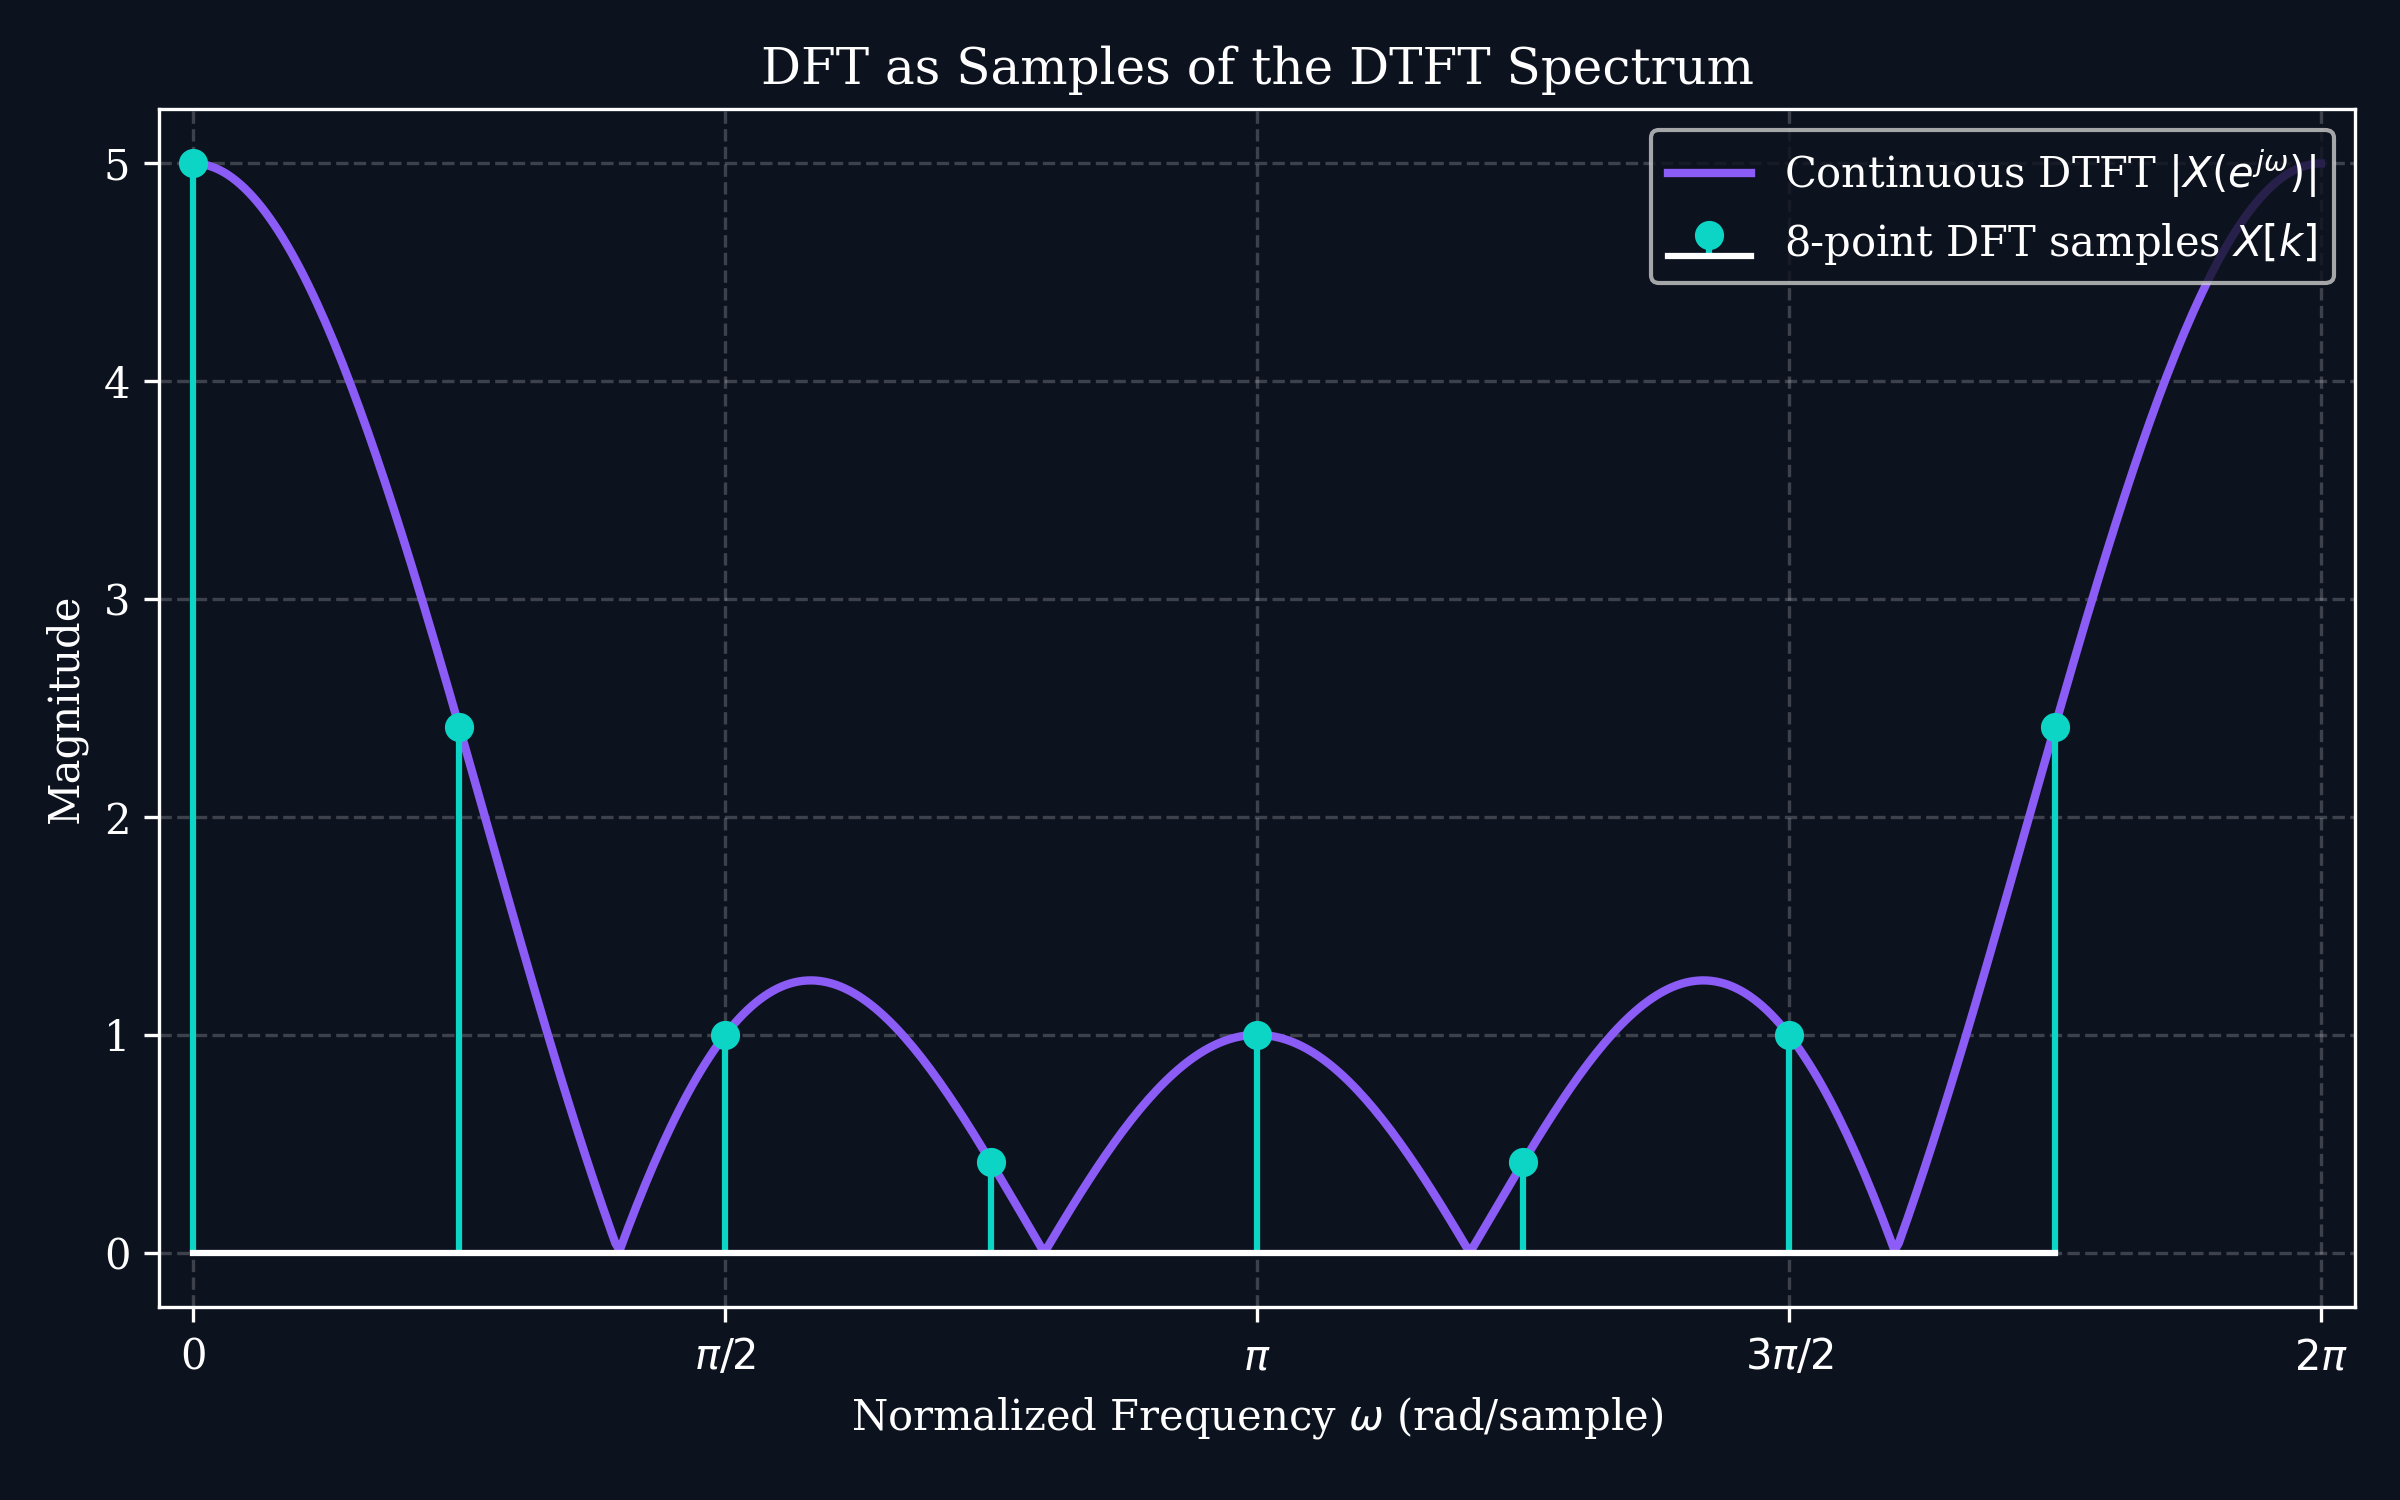
\includegraphics[width=0.85\textwidth]{images/dtft_vs_dft.png}
\caption{Sampling the continuous DTFT spectrum to obtain discrete DFT bins.}
\label{fig:dtft_vs_dft}
\end{figure}

\section{The Twiddle Factor and Its Properties}
To simplify notation, we introduce the \textbf{Twiddle Factor}:
\begin{equation}
W_N = e^{-j\frac{2\pi}{N}}
\end{equation}
The $N$-point DFT is defined as:
\begin{equation}
X[k] = \sum_{n=0}^{N-1} x[n] W_N^{kn}, \quad 0 \le k \le N-1
\end{equation}

\subsection{Properties of the Twiddle Factor}
\begin{enumerate}
    \item \textbf{Exponentiation to N:}
    \begin{equation*}
    W_N^N = \left(e^{-j\frac{2\pi}{N}}\right)^N = e^{-j2\pi} = 1 \implies W_N^{kN} = 1^k = 1
    \end{equation*}
    \item \textbf{Periodicity:}
    \begin{equation*}
    W_N^{k+N} = W_N^k \cdot W_N^N = W_N^k \cdot 1 = W_N^k
    \end{equation*}
    \item \textbf{Conjugate Symmetry:}
    \begin{equation*}
    W_N^{k(N-n)} = W_N^{kN} \cdot W_N^{-kn} = 1 \cdot (W_N^{kn})^{-1} = e^{j\frac{2\pi}{N}kn} = (W_N^{kn})^*
    \end{equation*}
\end{enumerate}

\section{Orthogonality Proof and IDFT Derivation}

\subsection{Orthogonality Proof}
Evaluate the sum of the product of two complex exponentials:
\begin{equation}
S = \sum_{n=0}^{N-1} W_N^{kn} W_N^{-ln} = \sum_{n=0}^{N-1} W_N^{(k-l)n}
\end{equation}
Let $m = k - l$. This is a geometric series $\sum_{n=0}^{N-1} (W_N^m)^n$.

\textbf{Case 1: $k = l$ (or $m = 0$)}\\
The ratio is $W_N^0 = 1$.
\begin{equation*}
S = \sum_{n=0}^{N-1} 1^n = N
\end{equation*}

\textbf{Case 2: $k \neq l$}\\
The geometric series sum formula gives:
\begin{equation*}
S = \frac{1 - (W_N^m)^N}{1 - W_N^m} = \frac{1 - W_N^{mN}}{1 - W_N^m} = \frac{1 - 1}{1 - W_N^m} = 0
\end{equation*}

\textbf{KEY RESULT: Orthogonality Condition}
\begin{equation}
\sum_{n=0}^{N-1} W_N^{kn} W_N^{-ln} = N \delta[k-l]
\end{equation}

\subsection{Derivation of the IDFT}
Starting with the DFT formula:
\begin{equation*}
X[k] = \sum_{m=0}^{N-1} x[m] W_N^{km}
\end{equation*}
Multiply both sides by $W_N^{-kn}$ and sum over $k$:
\begin{equation*}
\sum_{k=0}^{N-1} X[k] W_N^{-kn} = \sum_{k=0}^{N-1} \left( \sum_{m=0}^{N-1} x[m] W_N^{km} \right) W_N^{-kn}
\end{equation*}
Interchanging summation orders:
\begin{equation*}
\sum_{k=0}^{N-1} X[k] W_N^{-kn} = \sum_{m=0}^{N-1} x[m] \left( \sum_{k=0}^{N-1} W_N^{k(m-n)} \right)
\end{equation*}
By orthogonality, the inner sum is $N \delta[m-n]$:
\begin{equation*}
\sum_{k=0}^{N-1} X[k] W_N^{-kn} = x[n] \cdot N
\end{equation*}
Dividing by $N$ gives the Inverse Discrete Fourier Transform (IDFT):
\begin{equation}
x[n] = \frac{1}{N} \sum_{k=0}^{N-1} X[k] W_N^{-kn}, \quad 0 \le n \le N-1
\end{equation}

\section{Matrix Formulation of the DFT}
The DFT can be expressed as a matrix multiplication $\mathbf{X} = \mathbf{W}_N \mathbf{x}$:
\begin{equation}
\mathbf{W}_N = \begin{bmatrix}
1 & 1 & 1 & \dots & 1 \\
1 & W_N^1 & W_N^2 & \dots & W_N^{N-1} \\
1 & W_N^2 & W_N^4 & \dots & W_N^{2(N-1)} \\
\vdots & \vdots & \vdots & \ddots & \vdots \\
1 & W_N^{N-1} & W_N^{2(N-1)} & \dots & W_N^{(N-1)(N-1)}
\end{bmatrix}
\end{equation}

For $N=4$, with $W_4 = -j$:
\begin{equation}
\mathbf{W}_4 = \begin{bmatrix}
1 & 1 & 1 & 1 \\
1 & -j & -1 & j \\
1 & -1 & 1 & -1 \\
1 & j & -1 & -j
\end{bmatrix}
\end{equation}

The IDFT in matrix form is $\mathbf{x} = \frac{1}{N} \mathbf{W}_N^* \mathbf{X}$.

\begin{figure}[H]
\centering
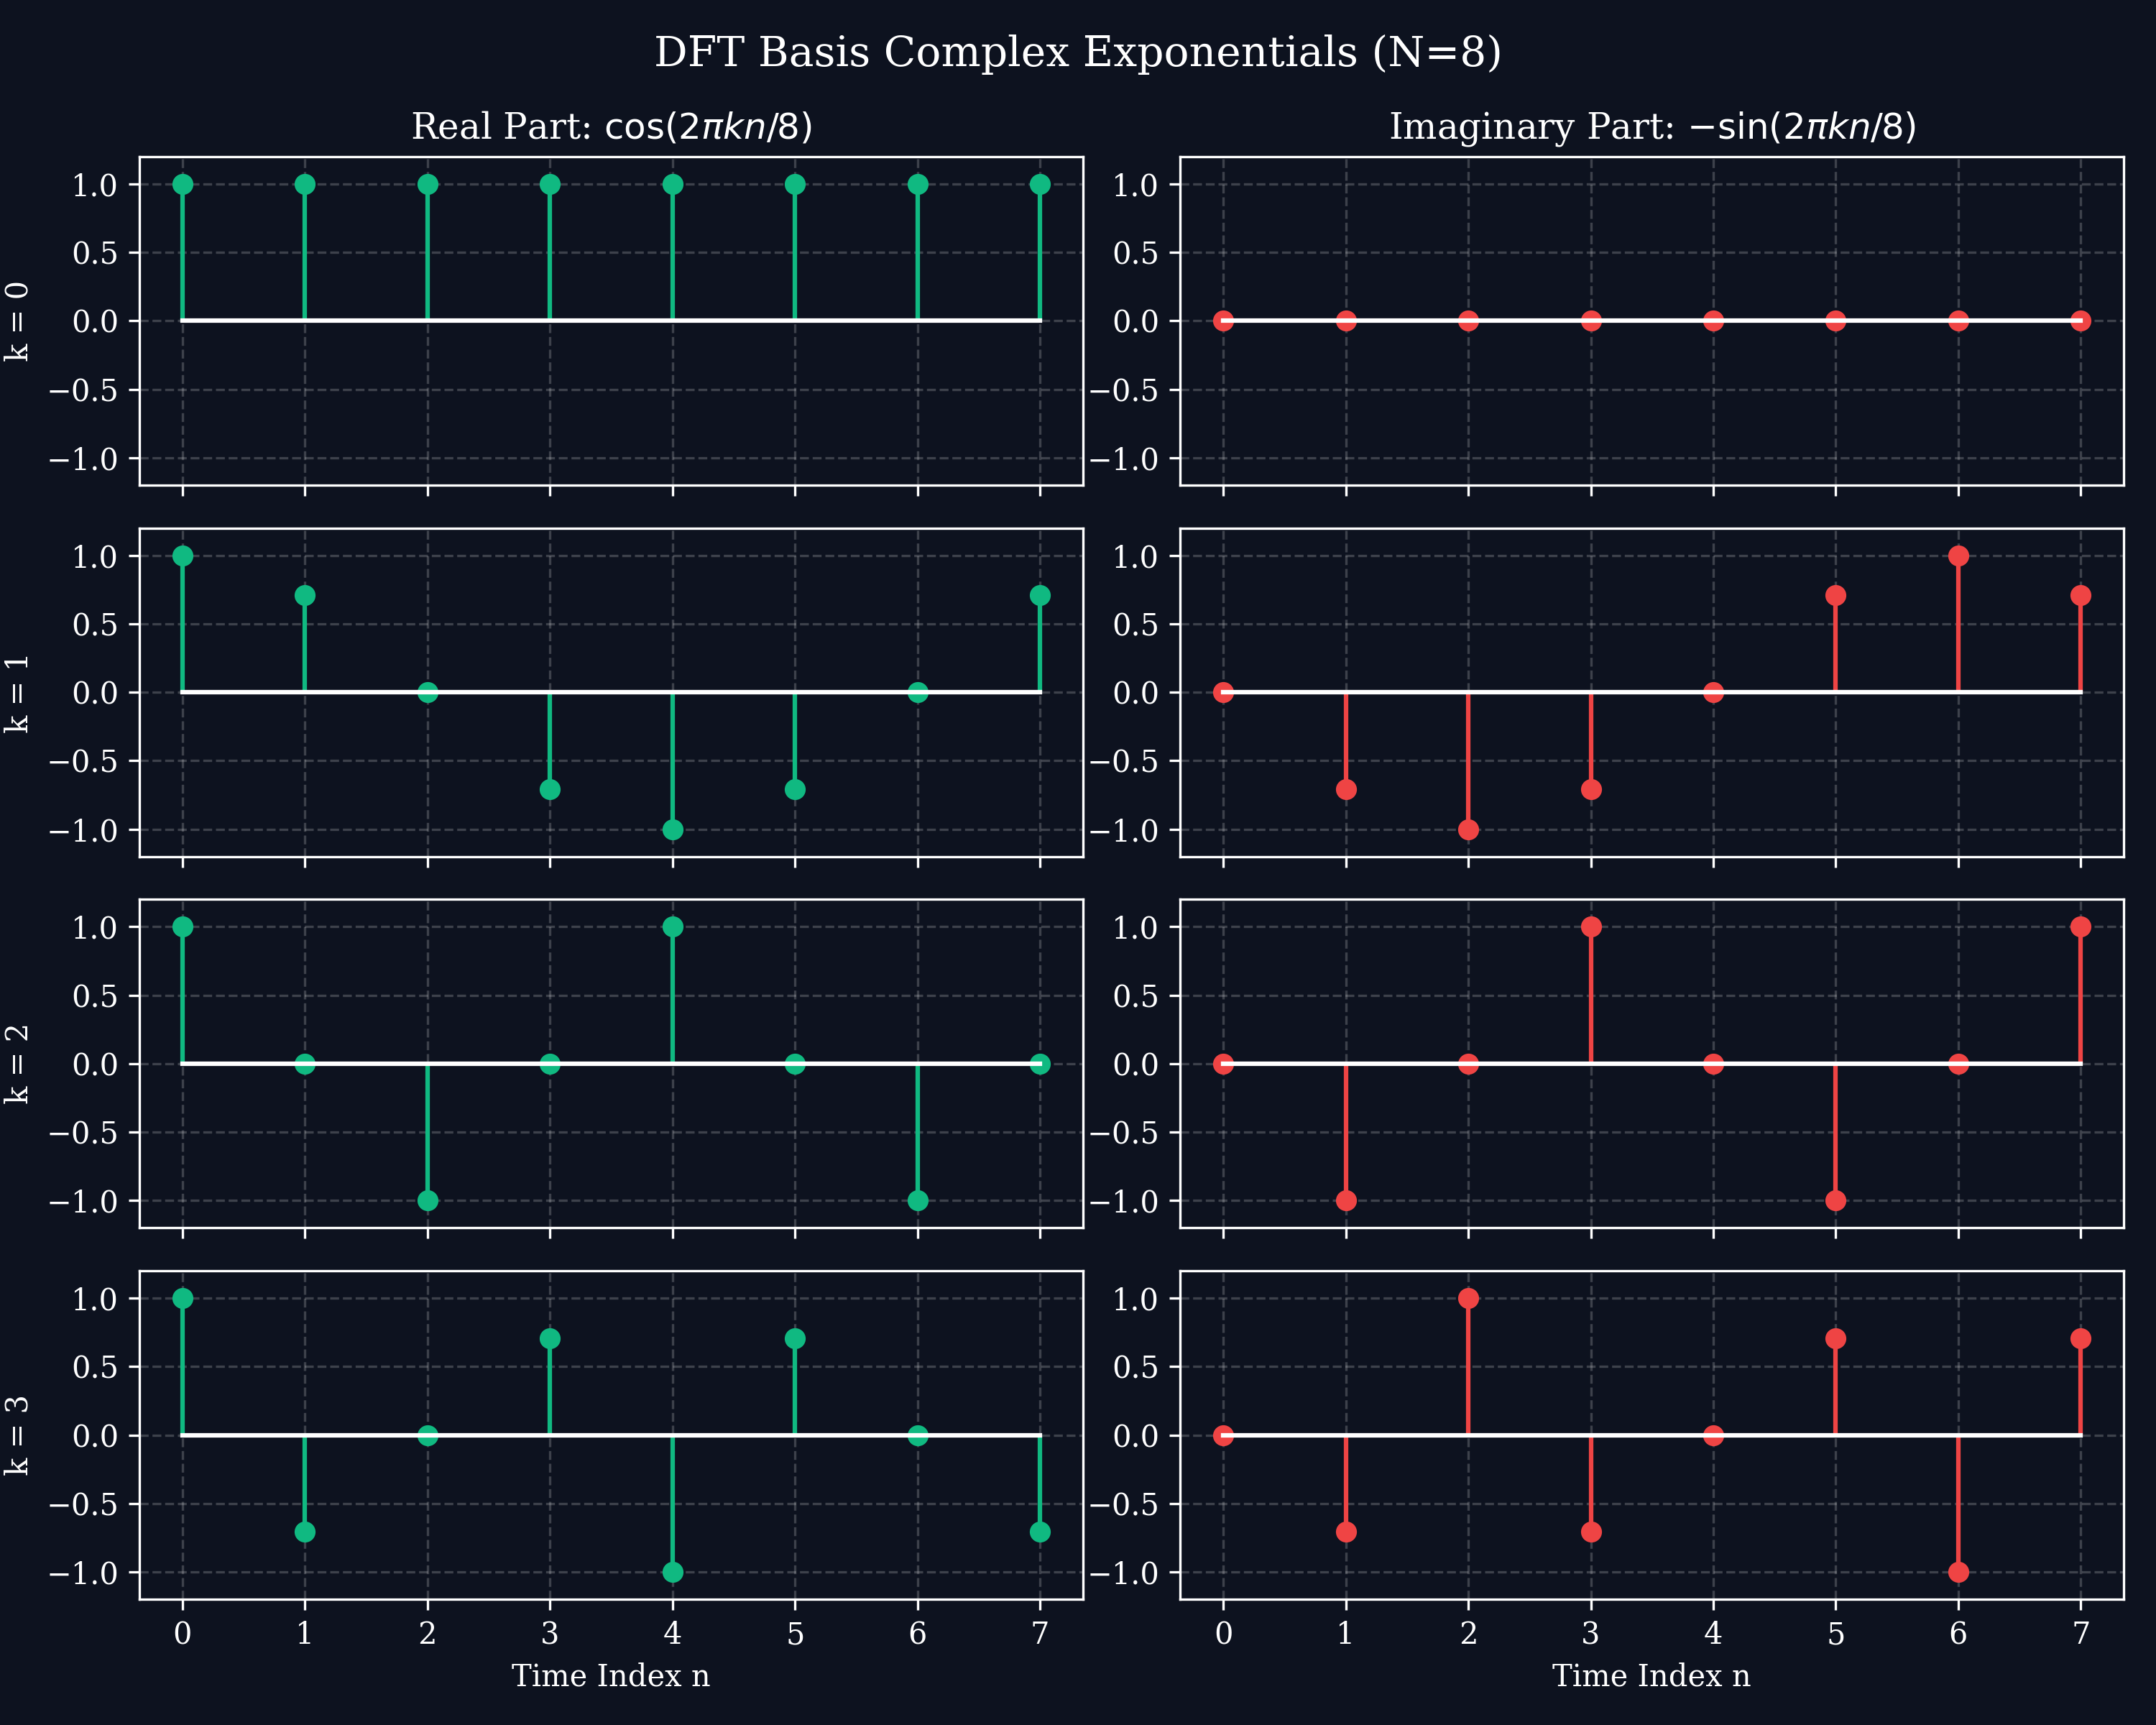
\includegraphics[width=0.85\textwidth]{images/dft_basis_functions.png}
\caption{Real and Imaginary basis functions for N=8.}
\label{fig:basis_vectors}
\end{figure}

\section{DFT of Common Sequences}
\begin{itemize}
    \item \textbf{Unit Impulse} $x[n] = \delta[n]$ $\implies X[k] = 1$ (Flat spectrum)
    \item \textbf{DC Sequence} $x[n] = 1$ $\implies X[k] = N \delta[k]$ (Zero-frequency spike)
    \item \textbf{Complex Exponential} $x[n] = e^{j\frac{2\pi}{N} m n}$ $\implies X[k] = N \delta[k-m]$
\end{itemize}

\section{Spectral Resolution and Zero-Padding}
The frequency resolution is $\Delta \omega = \frac{2\pi}{N}$ or $\Delta f = \frac{f_s}{N}$. To improve the \textit{display resolution} (making the spectrum appear smoother and denser), we can append zeros to the signal, increasing the DFT size $N$. Zero-padding interpolates the DTFT spectrum but does not improve the fundamental ability to resolve closely spaced frequencies.

\section{DFT Properties Table}
\begin{table}[H]
\centering
\begin{tabular}{lll}
\toprule
\textbf{Property} & \textbf{Time Domain $x[n]$} & \textbf{Frequency Domain $X[k]$} \\
\midrule
Linearity & $a x_1[n] + b x_2[n]$ & $a X_1[k] + b X_2[k]$ \\
Circular Time Shift & $x[(n - m) \pmod N]$ & $X[k] W_N^{km}$ \\
Circular Freq Shift & $x[n] W_N^{-ln}$ & $X[(k - l) \pmod N]$ \\
Circular Convolution & $x_1[n] \circledast x_2[n]$ & $X_1[k] X_2[k]$ \\
Conjugate Symmetry & If $x[n]$ is real & $X[k] = X^*[N-k]$ \\
\bottomrule
\end{tabular}
\end{table}

\section{Worked Example: Step-by-Step DFT Computation}
Find the 4-point DFT of $x[n] = \{1, 1, 0, 0\}$.
\begin{equation*}
\mathbf{X} = \mathbf{W}_4 \mathbf{x} = \begin{bmatrix}
1 & 1 & 1 & 1 \\
1 & -j & -1 & j \\
1 & -1 & 1 & -1 \\
1 & j & -1 & -j
\end{bmatrix} \begin{bmatrix} 1 \\ 1 \\ 0 \\ 0 \end{bmatrix}
\end{equation*}
\begin{align*}
X[0] &= 1(1) + 1(1) + 1(0) + 1(0) = 2 \\
X[1] &= 1(1) + (-j)(1) + (-1)(0) + j(0) = 1 - j \\
X[2] &= 1(1) + (-1)(1) + 1(0) + (-1)(0) = 0 \\
X[3] &= 1(1) + j(1) + (-1)(0) + (-j)(0) = 1 + j
\end{align*}
Result: $X[k] = \{2, 1-j, 0, 1+j\}$.

\section{Checkpoint Questions}
\begin{enumerate}
    \item \textbf{Prove that the 4-point DFT of $x[n] = \{1, -1, 1, -1\}$ is $X[k] = \{0, 0, 4, 0\}$.} \\
    \textbf{Ans:} The sequence is $\cos(\pi n) = (-1)^n = e^{j\pi n} = W_4^{-2n}$. This perfectly aligns with the $k=2$ basis vector. By orthogonality, the inner product yields $N=4$ at $k=2$ and $0$ elsewhere.
    \item \textbf{For a 1-second audio signal at 8000 Hz, how do you get 0.5 Hz DFT resolution?} \\
    \textbf{Ans:} $\Delta f = f_s / N \implies 0.5 = 8000 / N \implies N = 16000$. The signal has 8000 samples, so you must zero-pad by appending 8000 zeros.
    \item \textbf{If $x[n]$ is real and 8-point DFT $X[1] = 3+j2$, what is $X[7]$?} \\
    \textbf{Ans:} $X[7] = 3-j2$. By conjugate symmetry for real signals, $X[k] = X^*[N-k]$, so $X[7] = X^*[1]$.
\end{enumerate}

\end{document}
